\setchapterimage[2cm]{../images/header-sunflowers.jpg}
%\setchapterpreamble[u]{\margintoc}
\chapter{The sunflower molecules}
\labch{sunflowers}


\section{Introduction and origin}

The search for effective and interesting SERS substrates ended up leading us to a novel class of molecules researched and presented in the year 2006 by Chernichenko and his colleagues.\sidecite{chernichenko06}
The first representative of this family, nicknamed as \q{sulflower}, is the ocatathio[8]circulene.
This highly symmetric structure, which may be described as a form of carbon sulfide and as a belt of annulated thiophene cycles, is claimed to have great stability, high symmetry and unusual electronic properties.

\begin{marginfigure}
    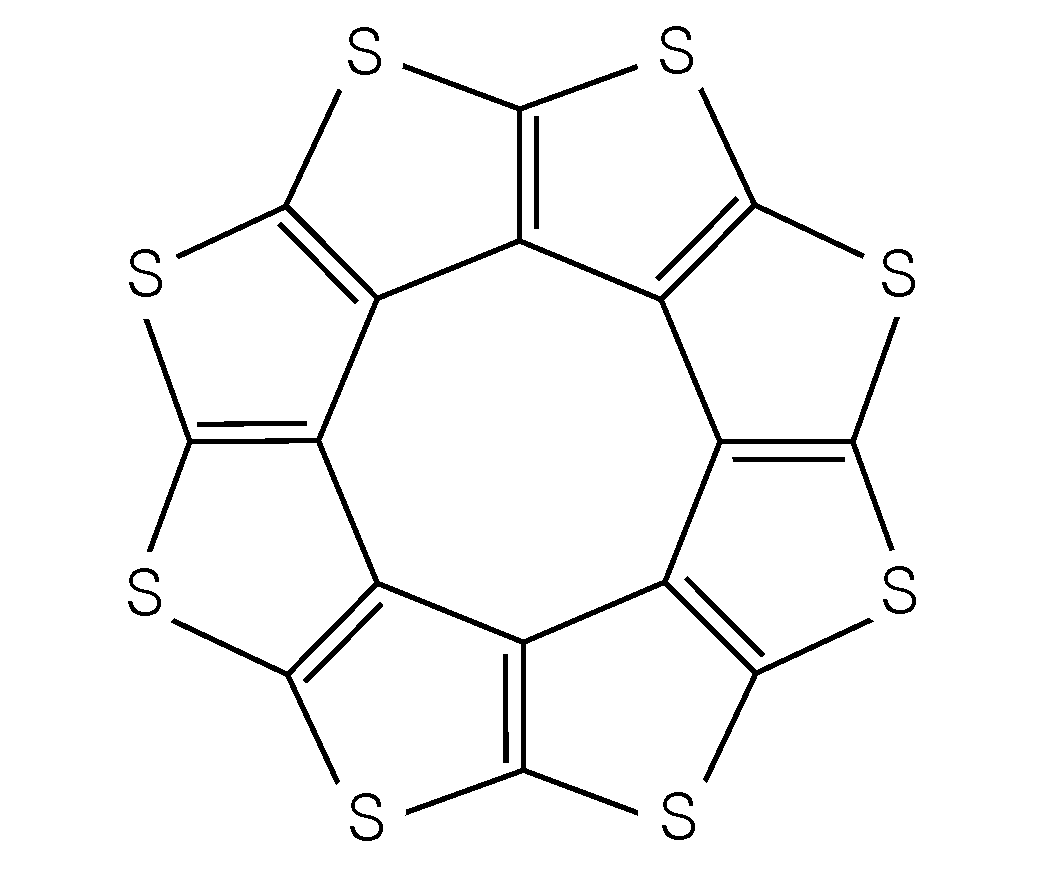
\includegraphics{sulflower-structure}
    \caption[Structure of sulflower]{Structure of sulflower}
    \labfig{sulflower-structure}
\end{marginfigure}


From a synthetic point of view, sulflower also proved to be simple and straightforward to develop despite its complex appearance: starting from tetrathiophene, sulphurizing its free sites and acidificating ot get polythiol, and removing the excess sulfur by vacuum pyrolysis.
This process allowed the team to achieve yields of 56\% starting from commercially available reagents.

Interestingly, the team proposes that it could be possible to prepare materials with diverse electronic properties by using different types of heteroatoms and varying on the basic structure of the molecule.
Such a statement made apparent the potential of this family of molecules: highly symmetrical, stable, surface-like structures with variable electronic behavior could act as suitable SERS substrates.
This chapter is entirely dedicated to that premise: the study and characterization of sulflower and sulflower-like molecules, which from now on I will collectively refer to as \q{sunflowers}.
By designing, generating and studying our own family of sunflowers, we will be contributing to characterize a novel and interesting group of molecules, and we may be able to identify an ideal SERS environment for STX.


\section{Sunflower design}

\begin{marginfigure}
    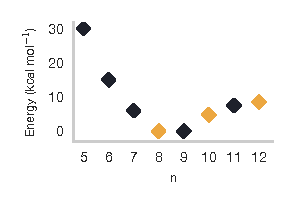
\includegraphics{sulflower-strain}
    \caption[Strain of thiophenic circulenes]{Strain of thiophenic circulenes with n rings}
    \labfig{sulflower-strain}
\end{marginfigure}

To start designing a family of molecules, first we must clearly state their defining pattern.
For this purpose, we adopt Chernichenko et al.'s own proposal: \q{a novel class of heterolytic circulenes}.
We start expanding the model by answering the question: are thiophene based circulenes with other than 8 rings stable enough to be worth considering?
The answer is in the original paper itself.
\reffig{sulflower-strain}, which was recreated to use our calculation level and adapt to the style of the document, shows that 8 ring structures are the most stable alongside 9.
The details about this calculation are further explained in \refsec{study-of-stability}.
However, considering their low relative energies and the fact that they have an even number of electrons (which would greatly simplify later calculations), 10 and 12 ring sunflowers were also chosen as part of the study.

Expanding upon this idea to allow for further heteroatom substitution, we ended up with the templates in \reffig{sunflower-skeletons}.
The possibilities were numerous, but we settled for S, Se, As and P substitutions on X$_1$ sites, and N substitutions in some cases in X$_2$ sites.
A full table detailing all of the structures that were generated and will comprise this study can be found in \reftab{sunflower-family}, as well as the short names or IDs that were given to each species based on its composition and number of petals for the sake of abbreviation.

\begin{figure*}
    \centering
    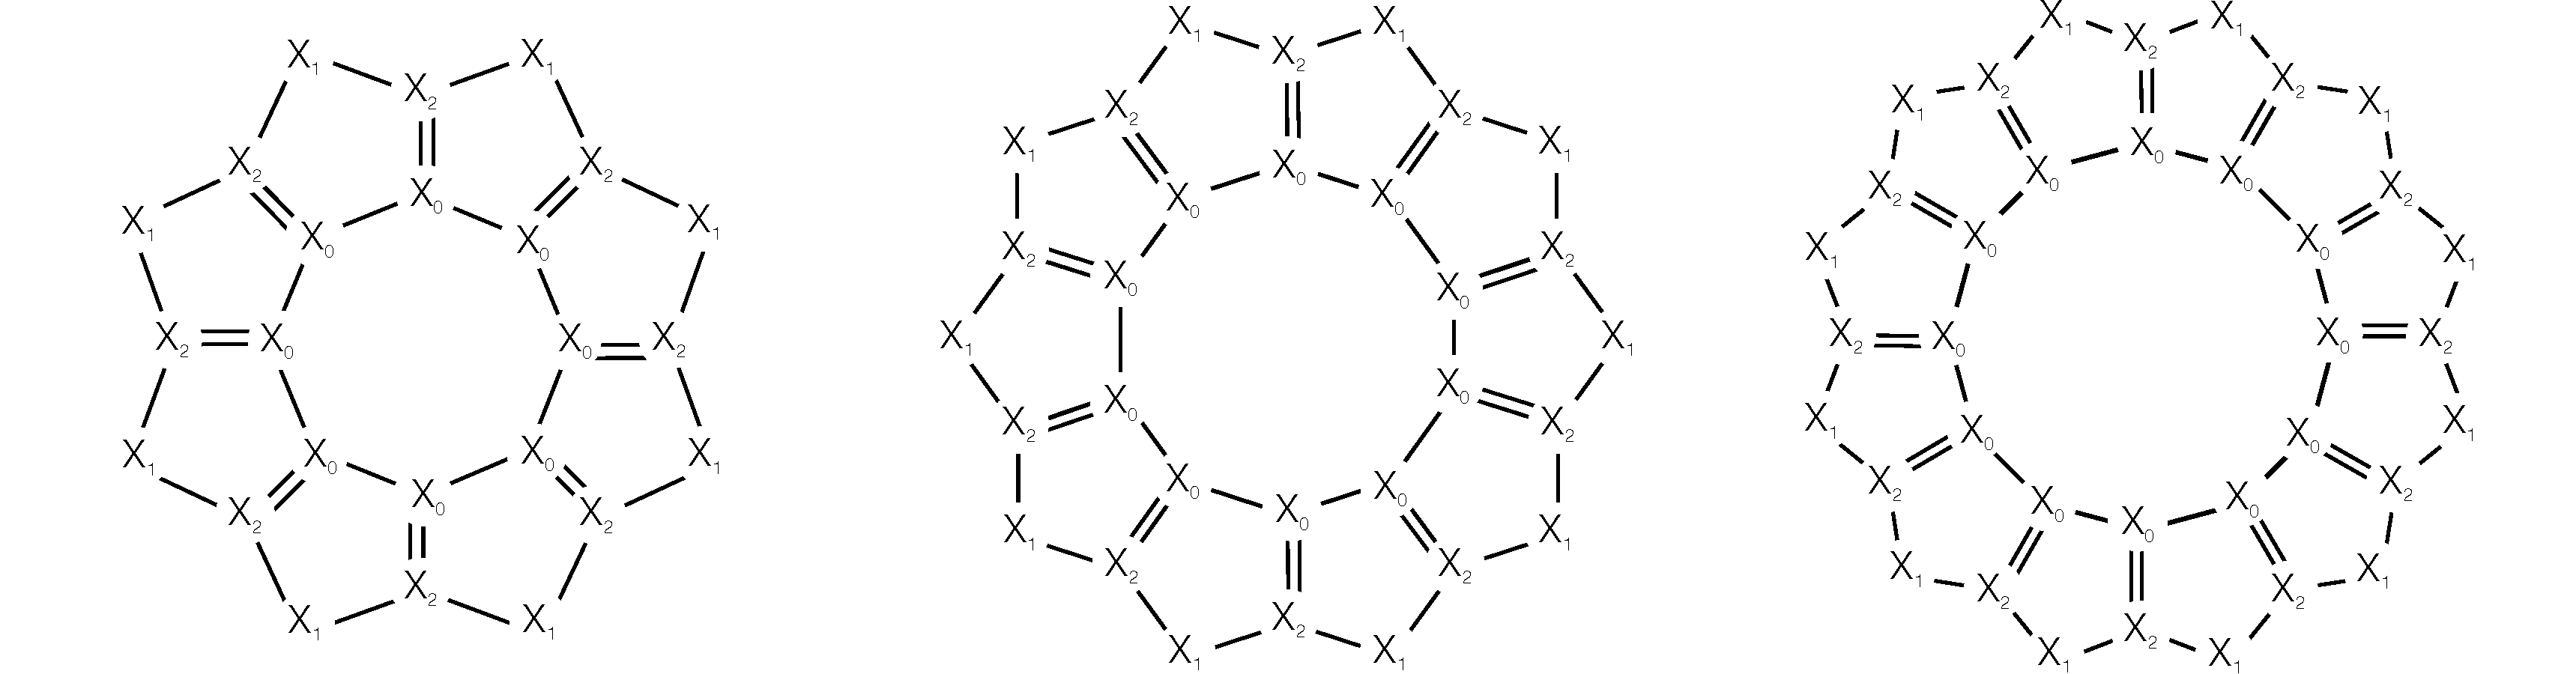
\includegraphics{sunflower-skeletons}
    \caption[General structures of the sunflower family]{From left to right, general structures of the 8, 10 and 12 ring sunflowers}
    \labfig{sunflower-skeletons}
\end{figure*}

\begin{table}
    \centering
    \caption[Sunflowers in this study]{Subset of the sunflower family that is going to be studied}
    \begin{tabular}{@{}cccrrr@{}}
        \toprule
        &&& \multicolumn{3}{c}{number of rings} \\
        X$_0$ & X$_1$ & X$_2$ & \multicolumn{1}{c}{8} & \multicolumn{1}{c}{10} & \multicolumn{1}{c}{12} \\
        \midrule
        C & S & C & S08 & S10 & S12 \\
        C & Se & C & Se08 & Se10 & Se12 \\
        C & As & C & As08 & As10 & As12 \\
        C & As & N & AsN08 & AsN10 & AsN12 \\
        C & P & C & P08 & P10 & P12 \\
        C & P & N & PN08 & PN10 & PN12 \\
        \bottomrule
    \end{tabular}
    \labtab{sunflower-family}
\end{table}

\section{Study of stability}
\labsec{study-of-stability}

Coordinate files for all of the designed sunflowers were created using 3D molecule modeling software.
Then, they were optimized at the M06-2X/def2SVP calculation level.

\blindtext

\begin{figure}
    \centering
    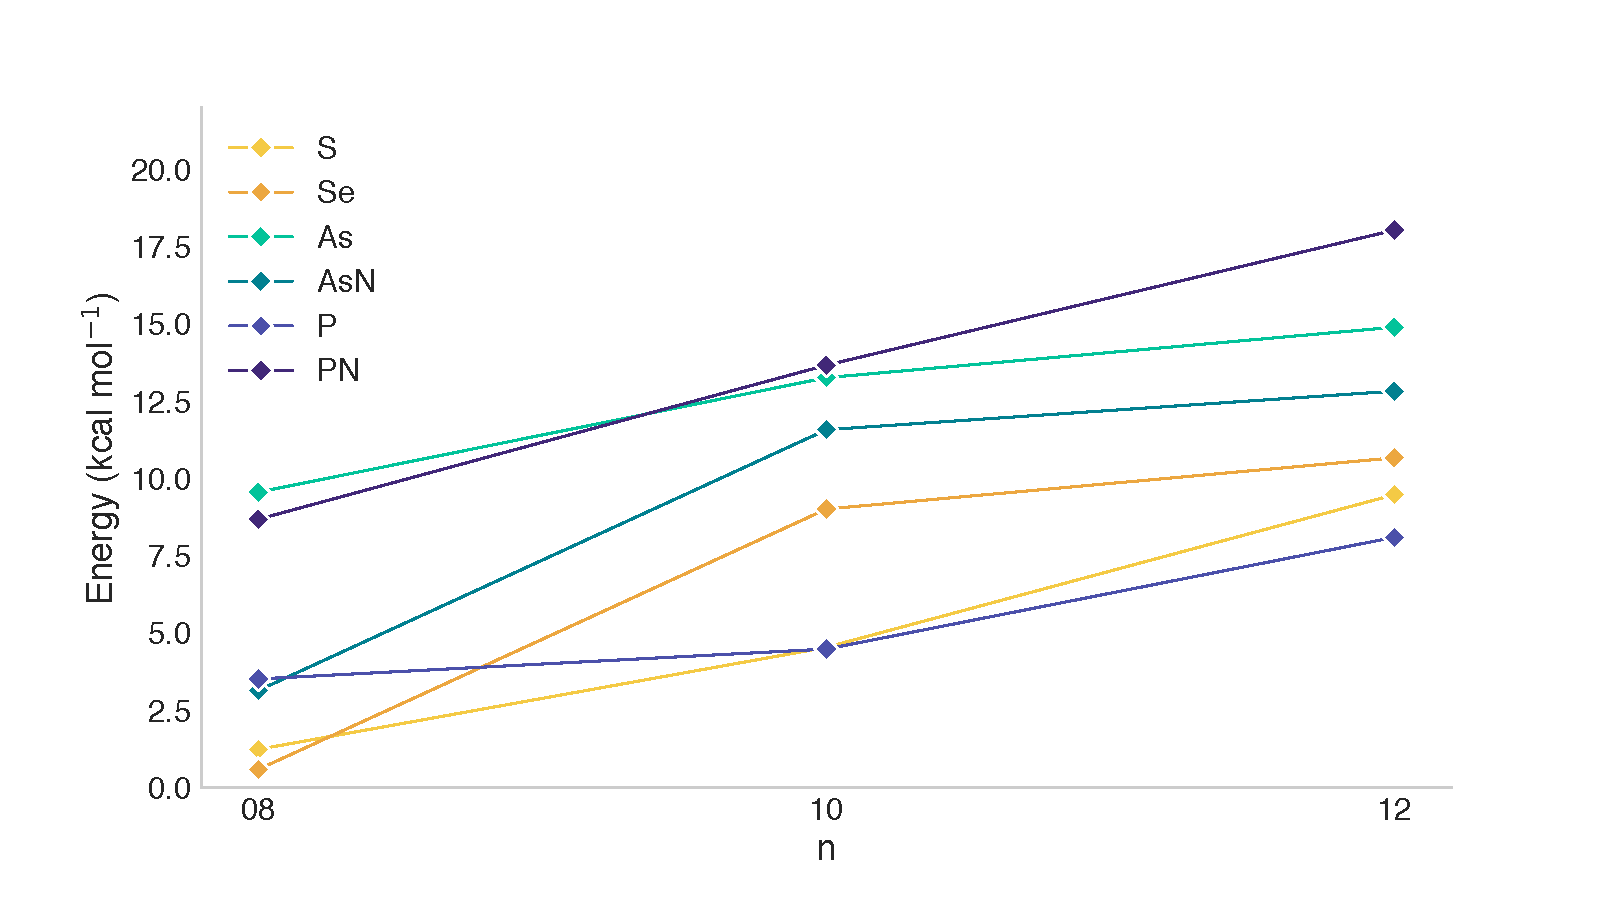
\includegraphics{sunflower-stability}
    \caption[Strain energies of sunflower groups]{Strain energies of all of the studied sunflower groups}
    \labfig{sunflower-stability}
\end{figure}

\blindtext

\section{Study of geometry}

\begin{marginfigure}
    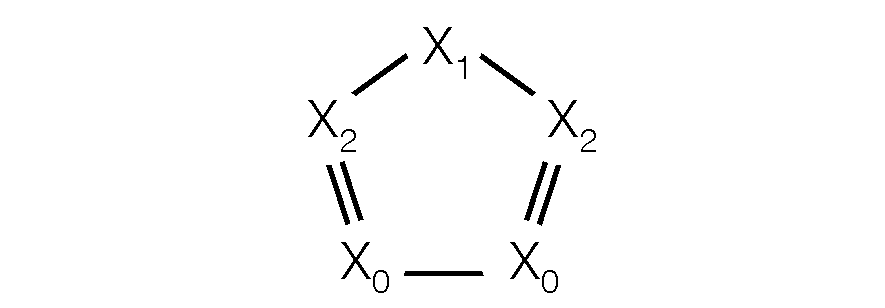
\includegraphics{pentagon-structure}
    \caption[Thiophene-like structure template]{Thiophene-like structure template (hydrogen is added to adjust for neutrality as needed)}
    \labfig{pentagon-structure}
\end{marginfigure}

Using the output files from the previous step, specifically from the initial optimization, bond length data was extracted using Python.
Then, the bonds were grouped by type: inner (I, bonds between X$_0$ atoms, which were carbon in all cases), middle (M, between X$_0$ and X$_2$ atoms, which were either C-C or C-N bonds), and outer (O, between X$_2$ and X$_1$ atoms).
The mean and standard deviation of these groups was computed for all of the systems.
Additionally, thiophene-like pentagonal structures of the form displayed in \reffig{pentagon-structure} were modeled and optimized, and their bond length data was compared with the rest.

\begin{table}
    \centering
    \caption[Bond length study]{Bond length statistics for each studied species, units are \si{\angstrom}}
    \begin{tabular}{@{}rlcccccc@{}}
        \toprule
        && \multicolumn{2}{c}{I (X$_0$-X$_0$)} & \multicolumn{2}{c}{M (X$_0$-X$_2$)} & \multicolumn{2}{c}{O (X$_1$-X$_2$)} \\
        && mean & std & mean & std & mean & std \\
        \midrule
        \multirow{4}{*}{S} & ring & 1.429 & - & 1.367 & 0.000 & 1.719 & 0.000 \\
        & 08 & 1.423 & 0.000 & 1.377 & 0.000 & 1.754 & 0.000 \\
        & 10 & 1.482 & 0.000 & 1.399 & 0.000 & 1.712 & 0.000 \\
        & 12 & 1.466 & 0.004 & 1.389 & 0.000 & 1.732 & 0.004 \\
        \\
        \multirow{4}{*}{Se} & ring & 1.434 & - & 1.363 & 0.000 & 1.857 & 0.000 \\
        & 08 & 1.454 & 0.000 & 1.385 & 0.000 & 1.865 & 0.000 \\
        & 10 & 1.478 & 0.003 & 1.389 & 0.000 & 1.861 & 0.004 \\
        & 12 & 1.466 & 0.007 & 1.381 & 0.000 & 1.877 & 0.005 \\
        \\
        \multirow{4}{*}{As} & ring & 1.468 & - & 1.354 & 0.000 & 1.918 & 0.000 \\
        & 08 & 1.434 & 0.050 & 1.448 & 0.000 & 1.859 & 0.008 \\
        & 10 & 1.436 & 0.000 & 1.454 & 0.001 & 1.856 & 0.001 \\
        & 12 & 1.435 & 0.042 & 1.446 & 0.002 & 1.867 & 0.007 \\
        \\
        \multirow{4}{*}{AsN} & ring & 1.495 & - & 1.283 & 0.000 & 1.854 & 0.000 \\
        & 08 & 1.434 & 0.000 & 1.361 & 0.000 & 1.858 & 0.000 \\
        & 10 & 1.450 & 0.001 & 1.364 & 0.001 & 1.856 & 0.004 \\
        & 12 & 1.440 & 0.004 & 1.357 & 0.001 & 1.873 & 0.006 \\
        \\
        \multirow{4}{*}{P} & ring & 1.467 & - & 1.359 & 0.000 & 1.794 & 0.001 \\
        & 08 & 1.410 & 0.048 & 1.445 & 0.000 & 1.764 & 0.006 \\
        & 10 & 1.431 & 0.000 & 1.471 & 0.000 & 1.736 & 0.000 \\
        & 12 & 1.429 & 0.045 & 1.462 & 0.002 & 1.747 & 0.005 \\
        \\
        \multirow{4}{*}{PN} & ring & 1.485 & - & 1.293 & 0.000 & 1.707 & 0.000 \\
        & 08 & 1.404 & 0.000 & 1.364 & 0.000 & 1.752 & 0.000 \\
        & 10 & 1.448 & 0.000 & 1.385 & 0.000 & 1.715 & 0.001 \\
        & 12 & 1.435 & 0.002 & 1.378 & 0.001 & 1.732 & 0.004 \\
        \bottomrule
    \end{tabular}
    \labtab{bond-length-study}
\end{table}

\section{Study of aromaticity}

Aromaticity is a property of molecules that have a ring or a chain of resonance bonds that increases their stability.
Initially associated with benzene, it’s typically found in flat ring structures (although there are other varieties such as homoaromatic and three-dimensional aromatic systems).

\subsection{Nucleus-Independent Chemical Shift (NICS)}

NICS

\subsubsection{The basics of NICS}

As $\pi$ electrons in aromatic systems have free circulation, an external magnetic field perpendicular to the main plane of the system is able to induce a ring current.
The NICS techinque as a probe for aromaticity is based on the idea that NMR chemical shifts are influenced by said ring currents, as a consequence of Ampère’s law.
Ring currents generate their own magnetic field, which will weaken or strengthen the effect of the external field resulting in decreased or increased shifts.
Aromatic systems will experience shielding on the inside of the ring and deshielding on the outside.
Antiaromatic systems will experience the opposite.

\subsubsection{A custom solution for non-planar molecules}
\blindtext

\subsection{AICD}
\subsubsection{The basics of AICD}
\blindtext
\subsubsection{Application and comparison of results}
\blindtext


\section{Spectroscopic characterization}

\subsection{Vibrational spectroscopy}
\subsubsection{Raman spectra}
\blindtext
\subsubsection{Decomposition of key modes}
\blindtext
\subsubsection{VEDA}
\blindtext

\subsection{Electronic spectroscopy}
\subsubsection{UV spectra}
\blindtext
